% !TeX encoding = UTF-8
% !TeX spellcheck = zh-cmn-Hans-CN
% !TeX program = xelatex
% !TeX root = ../main.tex

\documentclass[main.tex]{subfiles}

\begin{document}
\chapter{测度论}
本章我们将回顾一些测度论当中的一些定义与结论。如果读者没有接触过相关概念,那么可以将本章作为入门材料;如果读者已经有了相关知识,那么可以借本章做知识回顾之用。
一些比较困难的证明,特别是那些不符合直觉的,会放在附录中供读者参考。
如果读者拥有扎实的测度论基础,那么可以跳过\ref{sec:1.4}、\ref{sec:1.5}和\ref{sec:1.7}节,因为这些内容曾经是附录的一部分。

\section{概率空间} \label{sec:1.1}
书中的术语将以\textbf{粗体}标出。我们将从最基本的部分开始。
\term{概率空间}(probability space)是由表示``试验结果''的集合\(\Omega\) 、表示``事件''的集合\(\mathcal{F}\)和一个负责给事件分配概率的函数\(P:\mathcal{F} \rightarrow \intcc{0, 1}\)构成的三元组\((\Omega, \mathcal{F}, P)\)。
我们假定\(\mathcal{F}\)是一个\term{\(\sigma\)域}(\(\sigma\)-field)(又称\term{\(\sigma\)代数}(\(\sigma\)-algebra))\footnote{书中会根据语境将两者混用},是\(\Omega\)的(非空)子集族,并满足下列条件:
\begin{enumerate}
	\item \(A \in \mathcal{F} \Rightarrow A^c \in \mathcal{F}\)。
	\item \label{def:measure:2} 如果\(A_i \in \mathcal{F}\)是一个由可数个集合构成的集合列,那么\(\bigcup_i A_i \in \mathcal{F}\)。
\end{enumerate}

此处以及后文当中的\term{可数}(countable)表示基数为有限或可数无穷。由于\(\bigcap_i A_i = (\bigcup_i A_i^c)^c\),因此\(\sigma\)域在可数交下封闭。因此我们在定义中略去了该条性质以便简化验证\(\sigma\)域的过程。

如果没有\(P\),我们称\((\Omega, \mathcal{F})\)为\term{可测空间}(measurable space),即我们可以为该空间中指派一个测度。而\term{测度}(measure)是指非负的加性集函数,即符合下列条件的函数\(\mu: \mathcal{F} \rightarrow \R\)
\begin{enumerate}
	\item \(\forall A \in \mathcal{F}, \mu(A) \geq \mu(\emptyset) = 0\)
	\item 如果\(A_i \in \mathcal{F}\)是一个由可数个互不相交的集合构成的集合列,我们有
	\[\mu\left(\bigcup_i A_i\right) = \sum_{i}\mu(A_i)\]
	如果\(\mu(\Omega) = 1\),我们称这个\(\mu\)为\term{概率测度}(probability measure)。本书通常用\(P\)来表示概率测度。

	下面我们会从测度的定义出发推导一些在后文中常用结果。我们均认为下面提到的集合来自\(\mathcal{F}\)。
	\begin{theorem} \label{thm:1.1.1}
		令\(\mu\)为\((\Omega, \mathcal{F})\)上的测度
		\begin{enumerate}
			\item \label{prop:measure:monotone} \textbf{单调性} 如果 \(A \subseteq B\),那么\(\mu(A) \leq \mu(B)\)。
			\item \textbf{可数次可加性}\label{thm:1.1.1.2} 如果\(A \in \bigcup_{m=1}^\infty A_m\),那么\(\mu(A) \leq \sum_{m=1}^\infty\mu(A_m)\)。
			\item \label{prop:measure:below_continuity} \textbf{下连续性} % TODO: 这个翻译不好
			 如果\(A_i \uparrow A\)(即\(A_1 \subseteq A_2 \subseteq \dots\)且 \(\bigcup_i A_i = A\),那么就有 \(\mu(A_i) \uparrow \mu(A)\)。
			\item \textbf{上连续性} 如果\(A_i \downarrow A\)(即\(A_1 \supseteq A_2 \supseteq \dots\)且 \(\bigcap_i A_i = A\)且\(\mu(A_1) < \infty\),那么就有 \(\mu(A_i) \uparrow \mu(A)\)。
		\end{enumerate}
	\end{theorem}
	\begin{proof}
		\begin{enumerate}
			\item 用\(B-A = B\cap A^c\)表示二集合的\textbf{差集}。用\(+\)来表示集合的不交并,借助这些记号,我们就可以将\(B\)表示为\(A+(B-A)\),继而有
			\[\mu(B) = \mu(A) + \mu(B-A) \geq \mu(A)\]
			\item 令\(A^\prime_n = A_n \cap A, B_1 = A^\prime_1\),对于\(n > 1\)时,令\(B_n=A^\prime_n - \bigcup_{m=1}^{n-1}A^\prime_m\)
			注意到\(B_n\)互不相交,并且其并为整个\(A\),根据测度定义的性质\ref{def:measure:2}以及本定理的子句\ref{prop:measure:monotone}
			\[\mu(A) = \sum_{m=1}^{+\infty}\mu(B_m) \leq \sum_{m=1}^{+\infty}\mu(A_m)\]
			\item 令\(B_n = A_n - A_{n-1}\),那么\(B_n\)之间互不相交,并且有\(\bigcup_{m=1}^{+\infty} B_m = A, \bigcup_{m=1}^{n} B_m = A_n\),从而
			\[\mu(A) = \sum_{m=1}^{+\infty}\mu(B_m) = \lim\limits_{n\rightarrow +\infty}\bigcup_{m=1}^{n} B_m = \lim\limits_{n\rightarrow +\infty}\mu(A_n)\]
			\item 因为\(A_1 - A_n \uparrow A_1 - A\) 故由本定理的子句\ref{prop:measure:below_continuity}有\(\mu(A_1 - A_n) \uparrow \mu(A_1 - A)\)
			由于\(A_1\supseteq A\),故\(\mu(A_1 - A) = \mu(A_1) - \mu(A)\)从而有结果\(\mu(A_n)\downarrow\mu(A)\)
		\end{enumerate}
	\end{proof}
\end{enumerate}

最简单的例子就是本科概率论中的:
\begin{example}[离散概率空间] \label{ex:1.1.2} 令\(\Omega\)为某个可数集(即有限集或可数无穷集)。令\(\mathcal{F}=2^\Omega\)(即\(\Omega\)的所有子集之集)。并令
\[P(A) = \sum_{\omega \in A} p(\omega), \text{ 其中 } p(\omega) \geq 0 \text{ 且 } \sum_{\omega \in \Omega} p(\omega) = 1\]
我们不难发这个式子其实给出了离散概率空间上一般形式的概率测度。
在许多情形下\(\Omega\)会是有限集,且\(p(\omega) = 1/|\Omega|\),其中\(|\Omega|\)表示\(\Omega\)的基数。\footnote{中文教材中称这种情形为``古典概型''。}

对于可数集上一般形式的概率测度,有一个具体又简单的例子,就是 astragali\footnote{中国也有类似的东西,一般叫``羊拐''或``嘎拉哈''但用途不同。} ,源自古埃及,是一种用羊距骨制做的骰子。若投掷结果是用顶面朝上,则记为四点;若投掷结果是底面朝上,记为三点;由于骨头的两侧是经过打磨的,就是磨面相对较小,因此会存在磨面朝上的情况,这种情况记为六点;其他情况则记一点。
显然这四种情况的地位是不平等的,因此我们需要\(p_1, p_3, p_4\)和\(p_6\)来描述概率测度\(P\)。
\end{example}

在引入下个定义之前,我们需要先知道一个可以直接由\(\sigma\)-域的定义得到的结果:如果\(\mathcal{F}_i, i\in I\)是一个\(\sigma\)-域,那么\(\bigcap_{i\in I}\mathcal{F}_i\)也是一个\(\sigma\)-域。这里的\(I \neq \emptyset\)是任意指标集(也就是说,其可以为不可数集)。
从这个结果中我们可以知道,如果给定集合\(\Omega\)及其子集族\(\mathcal{A}\),那么存在包含\((\mathcal{A}\)的最小\(\sigma\)-域。我们称这个\(\sigma\)-域为\term{由\(\mathcal{A}\)生成的\(\sigma\)-域},并用记号\(\sigma(\mathcal{A})\)表示。

令\(\R^d\)为向量\((x_1, \dots, x_d), x_1, \dots, x_d\in \R\)构成的集合;\(\mathcal{R}^d\)为\term{博雷尔集},即包含所有\(\R^d\)开集的最小\(\sigma\)-域。当\(d=1\)时,上标通常会被略去。
\begin{example}[实直线上的测度]
	\((\R, \mathcal{R}^d)\)上的测度可以通过具有以下性质的\term{斯蒂尔切斯测度函数}(Stieltjes measure function)\(F\)来定义:
	\begin{enumerate}
		\item \(F\)不减
		\item \(F\)右连续,即\(\lim\limits_{y\downarrow x}F(y) = F(x)\)
	\end{enumerate}
\end{example}

\begin{theorem} \label{thm:1.1.4}
	存在\((\R, \mathcal{R})\)上的测度\(\mu\),使得
	\begin{equation} \label{eq:1.1.1}
		\mu(\intoc{a, b}) = F(b) - F(a)
	\end{equation}
\end{theorem}
若\(F(x) = x\),则称该测度为\term{勒贝格测度}(Lebesgue measure)。

\thmref{thm:1.1.4}的证明之路是漫长而又曲折的,因此我们只在此介绍一下本节当中会用到的一些想法,
而把具体细节放在附录的\ref{sec:a.1}节当中。
本定理之所以用``右闭区间''是因为如果\(b_n \downarrow b\),那么
\[\bigcap_{n} \intoc{a, b_n} = \intoc{a, b}\]
而下一个定理会解释为什么要采用``左开区间''。

如果集族\(\mathcal{S}\)符合:\begin{enumerate*}
	\item 其元素在交下封闭,即\(S, T \in \mathcal{S} \Rightarrow S \cap T \in \mathcal{S}\)
	\item 如果\(S \in \mathcal{S}\),那么\(S^c\)可以表示为由有限个\(\mathcal{S}\)中的不交的元素构成的并
\end{enumerate*},则称\(\mathcal{S}\)为\term{半代数}(semialgebra)。
半代数的一个重要例子是:
\begin{example} \label{ex:1.1.5}
	令\(\mathcal{S}_d\)由空集加上具有如下形式的集合构成:
	\[(a_1, b_1]\times\dots\times \intoc{a_d, b_d} \subseteq \R^d,\ \text{其中} -\infty \leq a_i < b_i \leq +\infty\]
\end{example}
式(\ref{eq:1.1.1})定义了半代数\(\mathcal{S}_1\)上的测度\(\mu\),为了从半代数过渡到\(\sigma\)-代数,我们需要借助一个中间产物。
称\(\Omega\)的子集族\(\mathcal{A}\)为一个\term{集(合)域}(field of sets)(或\term{集合上的代数}(algebra))\footnote{原文仅为field。且后文会混用。},如果\(A, B \in \mathcal{A} \Rightarrow A^c, A \cap B \in \mathcal{A}\)。由于\(A \cap B= (A \cup B)^c\),我们可以立即得到\(A \cap B \in \mathcal{A}\)。\(\sigma\)-域显然是一个集域。反之却不是,下面给出反例:

\begin{example}
	令\(\Omega = \mathbf{Z}\)为整数集。则\(\mathcal{A} = \{A: A \text{或} A^c \text{有限}\}\)是一个集域。
\end{example}

\begin{lemma} \label{lem:1.1.7}
	如果\(\mathcal{S}\)是一个半代数,那么\(\bar{\mathcal{S}} = \{\mathcal{S}\text{中元素的有限不交并}\}\)是一个集域,并称其为\term{由\(\mathcal{S}\)生成的集(合)域}。
\end{lemma}
\begin{proof}
	令\(A = +_i S_i\)以及\(B = +_j T_j\),其中\(+\)表示不交并,且指标集是有限集。我们有\(A \cap B = +_{i,j}S_i \cap T_j \in \bar{\mathcal{S}}\)。同样地,对于补运算,令\(A = +_{i}S_i\),有\(A^c = \bigcap_i S_i^c\),而\(\mathcal{S}\)的定义保证了\(S_i^c \in \mathcal{S}\)。从而\(\bar{\mathcal{S}}\)在交运算下是封闭的。因此\(\bar{\mathcal{S}}\)是一个集域。
\end{proof}

\begin{example}
	令\(\Omega = \R\)及\(\mathcal{S} = \mathcal{S}_1\),\(\mathcal{S}_1\)由空集以及下列形式的集合构成
	\[\bigcup_{i=1}^k \intoc{a_i, b_i}, \text{ 其中} -\infty \leq a_i < b_i \leq +\infty\]
	如果给定\(\mathcal{S}\)上的函数\(\mu\),我们可以通过
	\[\mu(+_{i=1}^{n} A_i) = \sum_{i=1}^{n}\mu(A_i)\]
	将其延拓到\(\bar{\mathcal{S}}\)上。
\end{example}

所谓\term{集(合)域\(\mathcal{A}\)上的测度},就是一个满足下列条件的函数\(\mu\):
\begin{enumerate}
	\item \(\forall A \in \mathcal{A}, \mu(A) \geq \mu(\emptyset) = 0\)
	\item 如果\(A_i \in \mathcal{A}\)互不相交且\emph{它们的并在\(\mathcal{A}\)中},那么
	\[\mu\left(\bigcup_{i=1}^{+\infty} A_i\right) = \sum_{i=1}^{+\infty} \mu(A_i)\]
\end{enumerate}
如果存在集合列\(A_n \in \mathcal{A}\),使得\(\mu(A_i) < +\infty\)且\(\bigcup_n A_n = \Omega\),则称\(\mu\)为\term{\(\sigma\)有限}。
令\(A^\prime_1 = A_1\)且对于\(n \geq 2\),
\[A^\prime_1 = \bigcup_{m=1}^n A_m \quad \text{或} \quad A^\prime_1 = A_n \cap \left(\bigcap_{m=1}^{n-1} A_m^c\right) \in \mathcal{A}\]
因此我们可以不失一般性地假定\(A_n \uparrow \Omega\)或\(A_n\)之间互不相交。

下面的结果将帮助我们把半代数\(\mathcal{S}\)上的测度延拓到它生成的\(\sigma\)代数上,即\(\sigma(\mathcal{S})\)上。
\begin{theorem} \label{thm:1.1.9}
	令\(\mathcal{S}\)为一个半代数并令\(\mu\)为定义在\(\mathcal{S}\)上的函数,且\(\mu(\emptyset) = 0\)。假设\begin{enumerate*}
		\item \label{thm:1.1.9.1} 如果\(S \in \mathcal{S}\)来自于有限个互不相交的\(S_i \in \mathcal{S}\)的并,那么\(\mu(S) = \sum_i \mu(S_i)\)
		\item \label{thm:1.1.9.2} 如果\(S_i, S \in \mathcal{S}\)且\(S = +_{i \geq 1} S_i\),那么\(\mu(S) \leq \sum_{i \geq 1} \allowbreak\mu(S_i)\)
	\end{enumerate*}。那么\(\mu\)有唯一的延拓\(\bar{\mu}\)使得其是\(\bar{\mathcal{S}}\),即由\(\mathcal{S}\)生成的集域,上的测度。
	如果\(\bar{\mu}\)是\(\sigma\)有限的,那么存在唯一的延拓\(\nu\),使得\(\nu\)为\(\sigma(\mathcal{S})\)上的测度。
\end{theorem}
在\ref{thm:1.1.9.2}及其后面的内容中,我们会用\(i \geq 1\)表示可数并,而单个的\(i\)或\(j\)表示有限并。由于本节内容使用了定理\ref{thm:1.1.9},因此该定理的证明放在了附录的\ref{sec:a.1}节当中。
为了验证定理中的条件\ref{thm:1.1.9.2}成立,用下面的结论会比较方便:
\begin{lemma} \label{lem:1.1.10}
	假定只有条件\ref{thm:1.1.9.1}成立。
	\begin{enumerate}[label*=(\alph*)]
		\item \label{lem:1.1.10.a} 如果\(A, B_i \in \bar{\mathcal{S}}\)并有\(A = +_{i=1}^n S_i\),那么\(\bar{\mu}(A) = \sum_{i=1}^n \bar{\mu}(B_i)\)。
		\item \label{lem:1.1.10.b} 如果\(A, B_i \subseteq \bar{\mathcal{S}}\)并有\(A = +_{i=1}^n S_i\),那么\(\bar{\mu}(A) \leq \sum_{i=1}^n \bar{\mu}(B_i)\)。
	\end{enumerate}
\end{lemma}
\begin{proof}
	从定义中我们可以得知,如果\(A = +_i B_i\)是由互不相交的\(S_i \in \bar{\mathcal{S}}\)构成的且\(B_i = +_j S_{i,j}\),那么
	\[\bar{\mu}(A) = \sum_{i,j} S_{i,j} = \sum_{i} \bar{\mu}(B_i) \]

	为了证明\ref{lem:1.1.10.b},我们从\(n = 1\)的情况开始,此时\(B_1 = B\)。由于\(B = A + (B \cap A^c)\)且\(B \cap A^c \in \bar{\mathcal{S}}\),所以
	\[\bar{\mu}(A) \leq \bar{\mu}(A) + \bar{\mu}(B \cap A^c) = \bar{\mu}(B)\]
	对于\(n > 1\)的情况,只需令\(F_k = B_1^c \cap \dots \cap B_{k-1}^c \cap B_k^c\),并且我们注意到
	\[\begin{split}
		\bigcup_i B_i &= F_1 + \dots + F_n\\
		A = A \cap \left(\bigcup_i B_i\right) &= (A \cap F_1) + \dots + (A \cap F_n)
	\end{split}\]
	故使用\ref{lem:1.1.10.a}、\(n = 1\)时的\ref{lem:1.1.10.b}并再次使用\ref{lem:1.1.10.a},我们便得到
	\[\bar{\mu}(A) = \sum_{k=1}^n \bar{\mu}(A \cap F_k) \leq \sum_{k=1}^n \bar{\mu}(F_k) = \bar{\mu}\left(\bigcup_i B_i\right)\]
\end{proof}
\begin{proof}[\thmref{thm:1.1.4}的证明]
	令\(\mathcal{S}\)为左开右闭区间\(\intoc{a,b}\),其中\(-\infty \leq a < b \leq +\infty\)。为了定义\(\mathcal{S}\)上的函数\(\mu\),
	我们从下面观察到的结果开始:
	\[F(+\infty) = \lim\limits_{x \uparrow +\infty} F(x)\quad \text{以及}\quad
	F(-\infty) = \lim\limits_{x \downarrow -\infty} F(x)\quad\text{存在}\]
	以及\(F(+\infty) > -\infty\)、\(F(-\infty) < +\infty\),故而当\(-\infty \leq a < b \leq +\infty\)时,\(\mu(\intoc{a, b}) = F(b) - F(a)\)是有意义的。

	如果\(\intoc{a, b} = +_{i=1}^{n}\intoc{a_i, b_i}\),那么我们一定可以重新排列区间相应端点的下标,使得\(a_1 = a, b_n = b\)以及对与\(2 \leq i \leq n\),我们有\(a_i = b_{n-1}\)。
	故\thmref{thm:1.1.9}中的条件\ref{thm:1.1.9.1}成立。
	下面验证条件\ref{thm:1.1.9.2},首先假定\(-\infty < a < b < +\infty\)和\(\intoc{a, b} \subseteq \bigcup_{i \geq 1} \intoc{a_i, b_i}\),其中(可不失一般性地认为)\(-\infty < a_i < b_i < +\infty\)。
	选择\(\delta > 0\)使得\(F(a + \delta) < F(a) + \epsilon\)以及\(\eta_i\)使得
	\[F(b_i + \eta_i) < F(b_i) + \epsilon 2^{-i}\]
	那么我们发现开区间\(\intoo{a_i, b_i + \eta_i}\)覆盖了有界闭区间\(\intcc{a + \delta, b}\),故存在有限子覆盖\(\intoo{\alpha_j, \beta_j}\),其中\(1 \leq j \leq J\)。
	由于\(\intoc{a + \delta, b} \subseteq \bigcup_{j=1}^J \intoo{\alpha_j, \beta_j}\),从\lemref{lem:1.1.10}的子句\ref{lem:1.1.10.b}意味着
	\[F(b) - F(a+\delta) \leq \sum{j=1}^J F(\beta_j) - F(\alpha_j) \leq \sum_{i=1}^{+\infty}(F(b_i+\eta_i) - F(a_i))\]
	根据我们选择的\(\delta\)以及\(\eta_i\),我们有
	\[F(b) - F(a) \leq 2\epsilon + \sum_{i=1}^{+\infty}(F(b_i+\eta_i) - F(a_i))\]
	由于\(\epsilon\)是任取的,故我们证明了当\(-\infty < a < b < +\infty\)时,定理是成立的。
	为了消除最后的障碍,只需注意到如果\(\intoc{a, b} \subseteq \bigcup_i \intoc{a_i, b_i}\)且对于当\(-\infty < A < B < +\infty\)时,有\(\intoc{A, B} \subseteq \intoc{a, b}\),那么我们有
	\[F(B) - F(A) \leq \sum_{i=1}^{+\infty} (F(b_i) - F(a_i))\]
	由于最后的结果对任意有界的\(\intoc{A, B} \subseteq \intoc{a, b}\)成立,故而我们得到了最终的结论。
\end{proof}
\subsubsection*{\(\R^{d}\)上的测度}
我们的下一个目标是将\thmref{thm:1.1.4}推广到\(\R^d\)上。我们首先得明确函数\(F\)需要满足的一些性质。模仿\(d = 1\)的情况,我们容易推断出\(F\)应该满足下列性质:
\begin{enumerate}
	\item \label{def:measure.Rd.1} \(F\)是不减的,即当\(x \leq y\)(意思是\(\forall i, x_i \leq y_i\))时,有\(F(x) \leq F(y)\)。
	\item \label{def:measure.Rd.2} \(F\)右连续,即当\(\lim\limits_{y \downarrow x} F(y) = F(x)\)(这里的\(x \downarrow y\)是指每个\(y_i \downarrow x_i\))。
	\item 如果\(x_n \downarrow -\infty\),即每个坐标分量\(x_i \downarrow -\infty\),那么\(\lim\limits_{n\rightarrow+\infty}F(x_n) = 0\)。
	如果\(x_n \uparrow -\infty\),即每个坐标分量\(x_i \uparrow +\infty\),那么\(\lim\limits_{n\rightarrow+\infty}F(x_n) = 1\)。
\end{enumerate}
但是此时情况却变了。考虑如下的\(F:\ \R^2 \mapsto \intcc{0, 1}\)
\[F(x_1, x_2) = \begin{cases}
	1 & \text{若}x_1, x_2 \geq 1\\
	\frac{2}{3} & \text{若}x_1 \geq 1 \text{且} 0 \leq x_2 < 1\\
	\frac{2}{3} & \text{若}x_2 \geq 1 \text{且} 0 \leq x_1 < 1\\
	0 & \text{其他}\\
\end{cases}\]
\begin{figure}
\centering
\begin{tikzpicture}[scale=2]
	\begin{scope}
		% probabilities
		\draw (.5,.5) node[anchor=base] {\huge $0$};
		\draw (-.5,.5) node[anchor=base] {\huge $0$};
		\draw (.5,-.5) node[anchor=base] {\huge $0$};
		\draw (-.5,1.5) node[anchor=base] {\huge $0$};
		\draw (1.5,-.5) node[anchor=base] {\huge $0$};
		\draw (-.5,-.5) node[anchor=base] {\huge $0$};
		\draw (1.5,.5) node[anchor=base] {\huge $\frac{2}{3}$};
		\draw (.5,1.5) node[anchor=base] {\huge $\frac{2}{3}$};
		\draw (1.5,1.5) node[anchor=base] {\huge $1$};

		% ticks
		\draw[xshift=1 cm,dashed] (0,2.2) -- (0,-1.2) node[below] {};
		\draw[yshift=1 cm, dashed] (2.2,0) -- (-1.2,0) node[left] {};
		\draw (1,0) node[anchor=north east] {$1$};
		\draw (0,1) node[anchor=north east] {$1$};

		% origin
		\draw (0,0) node[anchor=north east] {\Large $O$};

		% axes
		\draw[thick,->] (-1.2,0) -- (2.2, 0) node[below] {\Large $x_1$};
		\draw[thick,->] (0,-1.2) -- (0, 2.2) node[left] {\Large $x_2$};
	\end{scope}
\end{tikzpicture}
\caption{反例的示意图}
\label{fig:1.1}
\end{figure}
\figref{fig:1.1}给出了该反例的图像。
如果稍加思索,我们可以知道
\[\begin{split}
	\mu(\intoc{a_1, b_1} \times \intoc{a_2, b_2}) = &\mu(\intoc{-\infty,b_1} \times \intoc{-\infty,b_2}) - \mu(\intoc{-\infty,a_1} \times \intoc{-\infty,b_2})\\
&-\mu(\intoc{-\infty,b_1} \times \intoc{-\infty,a_2}) + \mu(\intoc{-\infty,a_1} \times \intoc{-\infty,a_2})\\
=&F(b_1, b_2) - F(a_1, b_2) - F(b_1, a_2) + F(a_1, a_2)
\end{split}\]
令\(\epsilon \rightarrow 0\), 把\(a_1=a_2=1-\epsilon\)和\(b_1=b_2=1\)带入上式,我们会发现
\[\mu(\intcc{1,1} = 1-\frac{2}{3}) - \frac{2}{3} + 0 = -\frac{1}{3}\]
用同样的方法,我们可以得到\(\mu(\intcc{1,0}) = \mu(\intcc{0,1})=2/3\)。

为了得到使\(F\)成为测度的第三个也是最后一个条件,令
\[\begin{split}
	A &= \intoc{a_1, b_1}\times\dots\times\intoc{a_d,b_d}\\
	V &= \{a_1, b_1\}\times\dots\times\{a_d,b_d\}
\end{split}\]
其中\(-\infty < a_i < b_i < +\infty\)。为了强调\(\infty\)不会出现在端点,我们称\(A\)为一个有限矩形。那么\(V\)就是矩形\(A\)的端点集。如果\(v \in V\),令
\[\begin{split}
	\sgn(v) &= (-1)^{v\text{中}a_i\text{的个数}}\\
	\Delta_A F &= \sum_{v \in V} \sgn(v)F(v)
\end{split}\]
若我们要让\(\mu(A) = \Delta_A F\),我们必须要假定
\begin{enumerate}
	\item[(iv)] \label{def:measure.Rd.4} 对所有的矩形\(A\),\(\Delta_A F \geq 0\)。
\end{enumerate}

\begin{theorem} \label{thm:1.1.11}
	假设\(F:\ \R^d \mapsto \intcc{0,1}\)满足上述条件\ref{def:measure.Rd.1}--\ref{def:measure.Rd.4}。
	那么\(\R^d, \mathcal{R}^d\)上存在唯一的测度\(\mu\),使得对于所有的有限矩形\(A\),有\(\mu(A) = \Delta_A F\)。
\end{theorem}

\begin{example}
	假设\(F(x) = \prod_{i=1}^{d}(F_i(x_i))\),其中\(F_i\)满足\thmref{thm:1.1.4}的条件\ref{def:measure.Rd.1}和条件\ref{def:measure.Rd.2}。
	此时,\[\Delta_A F = \prod_{i=1}^{d}(F_i(b_i) - F_i(a_i))\]
	当\(F_i(x) = x\)时,称该测度为\(\R^d\)上的勒贝格测度。
\end{example}
\begin{proof}
	令\(\mu(A) = \Delta_A F\)对所有有限矩形成立,然后利用单调性将其延拓到\(\mathcal{S}^d\)上。
	为了验证\thmref{thm:1.1.9}的条件\ref{thm:1.1.9.1},我们先引入一些概念。若点列符合\(a_i = \alpha_{i,0} < \alpha_{i,1} \dots < \alpha_{i,n} = b_i\)使得每个\(B_k\)可表示为
	\[\intoc{\alpha_{1,j_1-1, \alpha_{1,j_1}}} \times \dots \times \intoc{\alpha_{d, j_d-1},j_d}\quad \text{其中 } 1\leq j_i \leq n_i\]
	,则称\(A = +_k B_k\)为\(A\)的\term{正则细分}(regular subdivision)。
	容易看到,对于正则细分\(\lambda(A) = \sum_{k}\lambda(B_k)\)。(首先考虑所有断点是有限的情况,然后再将断点取极限就得到了一般结果。)
	为了将该结果推广到一般的有限细分\(A = +_j A_j\)上,只要将每个子矩形进行正则细分即可,这样我们就得到了\(A\)的正则细分。

	条件\ref{def:measure.Rd.2}的证明和\thmref{thm:1.1.4}如出一辙。为了保证与\thmref{thm:1.1.4}之证明记号的一致性\footnote{为了不与下标混淆,这里对于开覆盖取了上标。},对于\(x,y\in \R^d\),我们可以令
	\[\begin{split}
		\intoo{x,y} &= \intoo{x_1,y_1}\times \dots \times \intoo{x_d,y_d}\\
		\intoc{x,y} &= \intoc{x_1,y_1}\times \dots \times \intoc{x_d,y_d}\\
		\intcc{x,y} &= \intcc{x_1,y_1}\times \dots \times \intcc{x_d,y_d}
	\end{split}\]
	假设\(-\infty < a < b < +\infty\),这意味着每个每个端点都是有限的,并假设\(\intoc{a,b} \subseteq \bigcup_{i \geq 1} \intoc{a^i, b^i}\),其中(我们可以不失一般性地认为)\(-\infty < a^i < b^i < +\infty\)。
	令\(\bar{1} = (1,\dots,1)\),取\(\delta\)使得
	\[\mu(\intoc{a-\delta \bar{1},b}) > \mu(\intoc{a,b})\]
	并取\(\eta_i\)使得
	\[\mu(\intoc{a,b^i+\eta_i\bar{1}}) < \mu(\intoc{a^i, b^i}) + \epsilon 2^{-i}\]
	那么开矩形\(\intoo{a^i, b^i}\)会覆盖有界闭矩形\(\intcc{a+\delta\bar{1},b}\),那么必然存在子覆盖\(\intoo{\alpha^j, \beta^j}\),\(1 \leq j \leq J\)。
	由于\(\intoc{a+\delta\bar{1},b} \subseteq \bigcup_{j=1}^J \intoo{\alpha^j, \beta^j}\),\lemref{lem:1.1.10}的\ref{lem:1.1.10.b}意味着
	\[\mu(\intcc{a+\delta\bar{1},b}) \leq \sum_{j=1}^J \mu(\intoc{\alpha^j, \beta^j}) \leq \sum_{i=1}^{+\infty} \mu(\intoc{a^i, b^i+\eta_i\bar{1}})\]
	根据选择的\(\delta\)与\(\eta_i\)我们有
	\[\mu(\intoc{a,b}) \leq 2\epsilon + \sum_{i=1}^{+\infty} \mu(\intoc{a^i, b^i})\]
	由于\(\epsilon\)是任意的,我们就证明了该定理在\(-\infty < a < b < +\infty\)时的情形。
	为了完成证明,我们只需要重复在\thmref{thm:1.1.4}中的工作即可。
\end{proof}

\begin{figure}
\centering
\begin{tikzpicture}[scale=0.6]
	\begin{scope}
		% square
		\draw (0,0) -- (0,7) -- (7,7) -- (7,0) -- (0,0);

		\draw (0,3) -- (5,3);
		\draw (3,6) -- (5,6);

		\draw (2,0) -- (2,3);
		\draw (3,3) -- (3,7);
		\draw (5,0) -- (5,7);
	\end{scope}
\end{tikzpicture}
\hspace{1cm}

\begin{tikzpicture}[scale=0.6]
	\begin{scope}
		% square
		\draw (0,0) -- (0,7) -- (7,7) -- (7,0) -- (0,0);

		\draw (0,4) -- (7,4);
		\draw (0,3) -- (7,3);
		\draw (0,6) -- (7,6);
		\draw (2,0) -- (2,7);
		\draw (3,0) -- (3,7);
		\draw (5,0) -- (5,7);
	\end{scope}
\end{tikzpicture}
\caption{将细分转化为正则细分}
\end{figure}

\section*{习题}
\begin{exercise}
	\item 令\(\Omega = \R, \mathcal{F} = \{A\subseteq \R: A\text{或}A^c \text{可数}\}\)。当\(A\)可数时,\(P(A) = 0\),反之则\(P(A) = 1\)。
	证明\((\Omega, \mathcal{F}, P)\)是概率空间。
	\item 回顾\exref{ex:1.1.5}中\(\mathcal{S}_d\)的定义。
	证明\(\sigma(\mathcal{S}_d) = \mathcal{R}^d\),即由\(\R^d\)的博雷尔集构成的集族。
	\item 给定一个\(\sigma\)-域\(\mathcal{F}\),如果存在可数集\(\mathcal{C}\subseteq \mathcal{F}\)使得\(\sigma(\mathcal{C}) = \mathcal{F}\),则称\(\mathcal{F}\)是\term{可数生成的}(countably generated)。
	证明\(\mathcal{R}^d\)是可数生成的。
	\item \begin{enumerate*}
		\item 证明若\(\mathcal{F}_1 \subseteq \mathcal{F}_2 \subseteq \dots\)是\(\sigma\)-代数,则\(\bigcup_i \mathcal{F}_i\)是一个代数
		\item 举例说明\(\bigcup_i \mathcal{F}_i\)不一定是\(\sigma\)-代数。
	\end{enumerate*}
	\item 若对于一个集合\(A \subseteq \mathbf{N}^+\)有
	\[\lim\limits_{n \rightarrow +\infty} \frac{\envert{A \cap \{1,2,\dots,n\}}}{n} = \theta\]
	,则称集合\(A\)有\term{自然密度}(natural density)(又称\term{渐进密度}(asymptotic density))\(\theta\)。
	令\(\mathcal{A}\)是由自然密度存在的集合构成的集族。那么\(\mathcal{A}\)是\(\sigma\)域吗?是集域吗?
\end{exercise}

\section{分布} \label{sec:1.2}
当我们为概率空间定义随机变量的时候,事情会变得有意思起来。如果称定义在\(\Omega\)上的实值函数\(X\)满足\(\forall B\in \mathcal{R}, X^{-1}(B) = \{\omega: X(\omega) \in B\} \in \mathcal{F}\),则称\(X\)为\term{随机变量}(random variable)。有时为了加强\(\sigma\)域的存在感,我们会称\(X\)是\term{\(\mathcal{F}\)可测}的(\(\mathcal{F}\)-measurable)或记为\(X \in \mathcal{F}\)。
如果\(\Omega\)是一个离散概率空间(见\exref{ex:1.1.2}),那么任意函数\(X: \Omega \mapsto \R\)均为随机变量。
另一个平凡但实用的随机变量是集合\(A \in \mathcal{F}\)的\term{指示函数}(indicator function):
\[1_A(\omega) = \begin{cases}
	1 & \omega \in A\\
	0 & \omega \notin A
\end{cases}\]
这个记号的用意是提醒你它会将\(A\)中的元素映为\(1\)。分析学家通常叫它\(A\)的特征函数。不过要说明的是,在概率论中,这个术语被用于称呼另一个完全不同的东西(见\ref{sec:3.3}节)。

\begin{figure}[H]
\centering
\begin{subfigure}{.4\textwidth}
	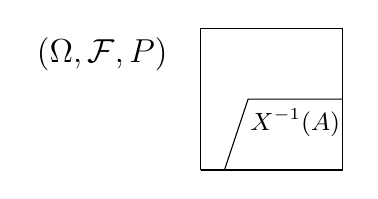
\begin{tikzpicture}[scale=0.3]
		\draw (-1,6) node[anchor=north east] {\large \((\Omega, \mathcal{F}, P)\)};
		\draw (0,0) -- (6,0) -- (6,6) -- (0,6) -- (0,0);
		\draw (1,0) -- (2,3) -- (6,3);

		\draw (4,1) node[anchor=south] {\small $X^{-1}(A)$};
	\end{tikzpicture}
\end{subfigure}
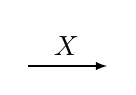
\begin{tikzpicture}
	\draw [-latex](0,0) -- (1,0);
	\node[text width=1em] at (0.5,0.25) {$X$};
\end{tikzpicture}
\begin{subfigure}{.4\textwidth}
	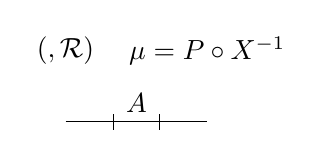
\begin{tikzpicture}[scale=0.3]
		\draw (0,0) -- (2,0);
		\draw [|-|](2,0) -- (4,0);
		\draw (4,0) -- (6,0);

		\draw (3,0) node[anchor=south] {\(A\)};
		\draw (0,2) node[anchor=south] {\((\R, \mathcal{R})\)};
		\draw (6,2) node[anchor=south] {\(\mu = P\circ X^{-1}\)};
	\end{tikzpicture}
\end{subfigure}
\caption{\(X\)的分布的定义}
\end{figure}
如果\(X\)是一个随机变量,那么通过对博雷尔集\(A\)定义测度\(\mu(A) = P(X \in A)\)诱导出的在\(\R\)上的概率测度称为\(X\)的\term{分布}(distribution)。
通过之前引入的记号,我们可以将等式右侧写成\(P(X^{-1}(A))\),也就是说我们先通过\(X^{-1}\)将博雷尔集\(A \in \mathcal{R}\)拉回到\(\sigma\)-域上的集合\(X^{-1}(A) \in \mathcal{F}\)上再通过概率测度\(P\)得到相应的概率。

为了验证\(\mu\)是概率测度,我们注意到如果\(A_i\)互不相交,那么通过\(\mu\)的定义,我们就知道\(X\)落在\(A_i\)的并中当且仅当\(X\)落在某个\(A_i\)中;也就是说,如果一组集合\(A_i \in \mathcal{R}\)是互不相交的,那么相应的事件\(\{X \in A_i\}\)也是互不相交的,再次借助\(\mu\)的定义,我们便有
\[\begin{split}
	&\mu\del{\bigcup_{i}A_i} = P\del{X \in \bigcup_{i}A_i}\\ =&P\del{\bigcup_{i} \{X \in A_i\}} = \sum_{i} P(X \in A_i) = \sum_i \mu(A_i)
\end{split}\]
我们一般是通过随机变量\(X\)的\term{分布函数}(distribution function),\(F(x) = P(X \leq x)\),来描述它的分布。

\begin{theorem} \label{thm:1.2.1}
	任何分布函数均有下列性质:
	\begin{enumerate}
		\item \label{thm:1.2.1.1} \(F\)不减。
		\item\label{thm:1.2.1.2} \(\lim\limits_{x \rightarrow +\infty} F(x) = 1\),\(\lim\limits_{x \rightarrow -\infty} F(x) = 0\)。
		\item\label{thm:1.2.1.3} \(F\)右连续,即\(\lim\limits_{y \rightarrow x^+} F(y) = F(x)\)。
		\item\label{thm:1.2.1.4} 若\(F(x^-) = \lim\limits_{y\rightarrow x^-}F(y)\)则\(F(x^-) = P(X < x)\)。
		\item\label{thm:1.2.1.5} \(P(X=x) = F(x) - F(x^-)\)。
	\end{enumerate}
\end{theorem}
\begin{proof}
	为了证明\ref{thm:1.2.1.1},只需注意到若\(x \leq y\)则有\(\{X \leq x\} \subseteq \{X \leq y\}\),之后使用\thmref{thm:1.1.1}的子句\ref{prop:measure:monotone}我们就可以得出\(P(X \leq x) \leq P(X \leq y)\)。

	为了证明\ref{thm:1.2.1.2},注意到若\(x \rightarrow +\infty\),则有\(\{X \leq x\} \uparrow \Omega\);同样地,我们还有若\(x \downarrow -\infty\),则有\(\{X \leq x\} \downarrow \emptyset\)。

	为了证明\ref{thm:1.2.1.3}只需注意到若\(y\downarrow x\)则\(\{X \leq y\} \downarrow \{X \leq x\}\)。

	为了证明\ref{thm:1.2.1.4}只需注意到若\(y\uparrow x\)则\(\{X \leq y\} \uparrow \{X \leq x\}\)。

	至于\ref{thm:1.2.1.5},只需注意到\(P(X = x) = P(X \leq x) - P(X < x)\),然后使用\ref{thm:1.2.1.3}和\ref{thm:1.2.1.4}即可。
\end{proof}

下一个结果将为我们进一步地刻画分布函数的性质。

\begin{theorem} \label{thm:1.2.2}
	如果\(F\)符合\thmref{thm:1.2.1}中的\ref{thm:1.2.1.1}、\ref{thm:1.2.1.2}和\ref{thm:1.2.1.3},那么它必然是某个随机变量的分布函数。
\end{theorem}
\begin{proof}
	令\(\Omega = \intoo{0,1}, \mathcal{F}=\Omega\)上的博雷尔集构成的集合,然后令\(P=\)勒贝格测度。若\(\omega \in \intoo{0,1}\),则令
	\[X(\omega) = \sup\{y:F(y) < \omega\}\]
	如果我们能证明
	\[\tag{$\star$}\label{thm:1.2.2.star}\{\omega: X(\omega) < x\} = \{\omega:\omega\leq F(x)\}\]
	那么我们就可以立即得到想要的结果,因为\(P(\omega:\omega\leq F(x)) = F(x)\)。(因为\(P\)在这里是勒贝格测度。)
	为了验证(\ref{thm:1.2.2.star}),我们注意到如果\(\omega'leq F(x)\),那么就有\(X(\omega) \leq x\),因为\(x \notin \{y: F(y) < \omega\}\)。
	如果\(\omega > F(x)\),从\(F\)的右连续性中可以得出,存在\(\epsilon > 0\)使得\(F(x+\epsilon) < \omega\)以及\(X(\omega) \geq x+\epsilon > x\)。
\end{proof}

即便\(F\)不是单射也不是满射(即不是双射),我们还是会称\(X\)为\(F\)的逆,并记为\(F^{-1}\)。
证明\thmref{thm:1.2.2}所用到的方法被广泛应用于计算机中随机变量的生成。
首先生成一个具有均匀分布的随机变量\(U\),然后借助\thmref{thm:1.2.2}中构造的\(F\)来得到一个新的随机变量\(F^{-1}(U)\),显然其分布函数就是\(F\)。

如果\(X\)和\(Y\)在\((\R,\mathcal{R})\)上诱导除了相同的分布\(\mu\),我们就称\(X\)和\(Y\)是\term{在分布意义下相等}(equal in distribution)的。
在\thmref{thm:1.1.4}的观点下,\(X\)和\(Y\)在分布意义下相等当且仅当\(X\)和\(Y\)具有相同的分布,人们通常会记为
\[X \stackrel{d}{=} Y\]
但是这个记号在本中显得太长了,出于印刷等方面的因素我们会使用记号\(X =_d Y\)。

当一个分布函数\(F(x) = P(X \leq x)\)具有如下形式:
\begin{equation}\label{eq:1.2.1}
	F(x) = \int_{-\infty}^{x}f(y) \dif y
\end{equation}
则称\(X\)具有\term{密度函数}(density function)\(f\)。为了方便记忆,我们可以认为\(f(x)\)就``代表''了\(P(X=x)\),然而实际上却是
\[P(X = x) = \lim\limits_{\epsilon \rightarrow 0}\int_{x-\epsilon}^{x+\epsilon} f(y) \dif y = 0\]
出于一般性的考量,我们不会使用诸如\(P(X=x)\)的记号来表示密度函数。取而代之的是另一个更具启发意义的记号\(f_X(x)\)。

因此我们可以借助\(f\)和式\eqref{eq:1.2.1}来定义分布函数\(F\)。为了让其结果是分布函数,其充分必要条件为\(f(x) \geq 0\)且\(\int_\R f(x) \dif x = 1\)。
下面展示三个比较重要的例子:
\begin{example}[\(\intoo{0,1}\)上的均匀分布]
	若\(x \in \intoo{0,1}\),则\(f(x) = 1\),其他情况则为\(0\)。
	其分布函数为:
	\[F(x) = \begin{cases}
		0&x\leq 0\\
		x&0\leq x\leq 1\\
		1&x>1
	\end{cases}\]
\end{example}
\begin{example}[率参数为\(\lambda\)的指数分布]
	若\(x \geq 0\)则\(f(x) = \lambda e^{-\lambda x}\)其他情况则为\(0\)。
	其分布函数为
	\[F(x) = \begin{cases}
		0&x\leq 0\\
		1-e^{-\lambda x}&x \geq 0
	\end{cases}\]
\end{example}
\begin{example}[标准正态分布]
	\[f(x) = (2\pi)^{-1/2}\exp(-x^2/2)\]
\end{example}
此时\(F\)并没有所谓的闭合式,但是针对比较大的\(x\),它的分布有如下形式的界:
\begin{theorem}
	对\(x > 0\)
	\[(x^{-1} - x^{-3})\exp(-x^2/2) \leq \int_{x}^{+\infty} \exp(-y^2/2) \dif y \leq x^{-1}\exp(-x^2/2)\]
\end{theorem}
\begin{proof}
	做换元\(y=x+z\)并用不等式\(\exp(-z^2/2) \leq 1\),我们有
	\[\int_{x}^{+\infty} \exp(-y^2/2) \dif y \leq \exp(-x^2/2)\int_{0}^{+\infty}\exp(-xz) \dif z = x^{-1}\exp(-x^2/2)\]
	对于不等式的另一侧,注意到
	\[\int_{x}^{+\infty} (1-3y^{-4})\exp(-y^2/2) \dif y = (x^{-1} - x^{-3})\exp(-x^2/2)\]
\end{proof}
如果一个\(\R\)上的分布函数具有密度,。有关这些记号的更多内容请参考\secref{sec:a.4}。
一个奇异分布的例子是:
\begin{example}[康托尔集上的均匀分布]\label{ex:1.2.7}

\end{example}
\section{随机变量} \label{sec:1.3}
\section{积分} \label{sec:1.4}
\section{积分的性质} \label{sec:1.5}
\section{期望值} \label{sec:1.6}
\section{积测度、富比尼定理} \label{sec:1.7}
\begin{exercise}
	\item
	\item
	\item
	\item \label{e1.7.4}
\end{exercise}
\end{document}
